\documentclass[12pt]{article}

% ---
% PACOTES
% ---
\usepackage{lmodern}			
\usepackage[T1]{fontenc}		
\usepackage[utf8]{inputenc}
\usepackage[brazilian]{babel}
\usepackage{indentfirst}		
\usepackage{color}				
\usepackage{graphicx}			
\usepackage{microtype} 			
\usepackage{lipsum}	
\usepackage{hyperref}
\usepackage{setspace}
\usepackage{multirow}
\usepackage{blindtext}
\usepackage{enumitem}

	
\usepackage{float}
\usepackage[hmarginratio=1:1]{geometry}

\usepackage[font={small},figurename={Figura},tablename=Tabela]{caption}
\usepackage{longtable}


% ------------------------------------------
% Configurações
% ------------------------------------------
\addto\captionsbrazilian{
  \renewcommand{\contentsname}%
    {Sumário}%
}


\begin{document}

% ------------------------------------------
% Sumário
% ------------------------------------------
\tableofcontents

\newpage
\begin{doublespacing}

\section{Guia de termos}
\begin{enumerate}
	\item{\textbf{ repositório:} um diretório controlado por git. Pode ser local (um diretório no seu computador) ou remoto (github, gitlab, etc).}
branch: é uma ramificação do seu projeto, você pode criar ramos, trocar o branch que você está controlando no momento ou fundir (dar merge em) dois branches. Olhe os itens 7, 8, 9 e 10 do exemplo de fluxo abaixo.
\item{\textbf{master:} é o ramo (branch) mais importante do projeto, imagine ele como o tronco da árvore e os outros branches são os ramos que saem dele. Idealmente, tudo que está no master são versões do código que já foram testadas em outros branches e depois fundidas com o master ou antes de terem sido adicionadas ao git em um commit.}
	\item{\textbf{HEAD:} é o último commit do branch que você está controlando no momento. Imagine que você acabou de chegar em um checkpoint de um jogo, e tem alguma coisa que indica que aquele foi o último save que você deu caso você tente carregar o jogo. O HEAD é parecido, ele GERALMENTE mostra qual foi o último commit que você deu no branch atual. Se você mudar pra outro branch, ele atualiza o HEAD pro último commit desse branch, se você der um commit o HEAD vai pra esse novo commit.}
\item{\textbf{origin}: é o repositório remoto que seu repositório local usa de referência. Basicamente, é na origin que você publica o código que vocÊ alterou e adicionou ao git localmente e busca códigos feitos por outras pessoas para modificar localmente.}

\end{enumerate}

\section{Fluxo comum de uso de git}
\subsection{Primeira vez que for usar}
O git usa seu nome e email para manter informações de quem está dando commits em algum projeto. Por isso, a primeira vez que você for usar git em uma conta nova do seu computador (ou na sua conta no IC, por exemplo), você vai precisar dizer quem é você e qual seu email. Apenas utilize os seguintes comandos:
\begin{flushleft}
\textit{\$ git config $--$global user.email <seuemail@examplo.com> \newline
\$ git config $--$global user.name <seu lindo nome>}
\end{flushleft}

\subsection{Lista de comandos}
\label{comandos}
\begin{enumerate}

\item{Criamos um repositório git \newline
\textit{\$ git init}
}  
\item{Adicionamos um repositório remoto (origin) \newline
\textit{\$ git remote add origin <url do repositório remoto>}
}

\item{Copiamos o que existe na origin \newline
\textit{\$ git pull origin <nome do branch, normalmente usamos o master> }
}
\item{Adicionamos arquivos ao git \newline
\textit{\$ git add <nome dos arquivos ou diretórios>}
}
\item{Utilizamos commit para efetivar as últimas mudanças (como salvar um checkpoint) \newline
\textit{\$ git commit -m “ Sua mensagem de commit aqui ”}
}
\item{Mantemos uma visão do estado atual do repositório \newline
\textit{\$ git status}
}
\item{Criamos eventuais branches (ramos) \newline
\textit{\$ git branch <nome do branch>}
}
\item{Alteramos o branch que estamos modificando (como dar load em um checkpoint). \newline
	\textit{\$ git checkout <nome do branch>  }
}
\item{Mantemos uma visão do estado da nossa árvore de commits e branches \newline
\textit{\$ git log}
}
\item{Efetuamos merges dos branches com nosso master \newline
	\textit{\$ git checkout <branch que você quer manter, normalmente o master> \newline
    \$ git merge <nome do branch que você está dando merge>}
}
\item{Atualizamos nossa origin com as mudanças \newline
	\textit{\$ git push origin master}
}
\end{enumerate}

\subsection{Importante saber sobre os comandos}
\begin{itemize}

\item{Os itens 6 e 10 podem (e devem) ser executados o tempo todo para verificar se o repositório está do jeito que você acredita que esteja
}
\item{Os itens da seção \ref{comandos} listam um fluxo razoavelmente completo do uso de git, nem sempre passamos por todas essas etapas, principalmente em projetos pequenos como um lab de mc202 =)
}

\item{No item 12 podemos colocar outros branches além do master na nossa origin, isso é comum quando nossos branches são grandes e temos mais de uma pessoa trabalhando neles
}

\item{\textbf{IMPORTANTE} - No item 11 podem ocorrer erros de conflito (imaginem que no master um arquivo tem uma linha X e no branch o mesmo arquivo não tem essa linha, qual das versões o git deve utilizar?). Podemos corrigir os conflitos na mão ou utilizar alguma flag para o git decidir qual versão usar (esse link explica bem como lidar com conflitos: https://www.git-tower.com/learn/git/faq/solve-merge-conflicts)
}

\item \textbf{IMPORTANTE} - No item 8 dos examplos anteriores, também podemos dar checkout para um commit passado (imagine que você descobriu um problema no último commit). Porém, essa não é a melhor prática de git, o ideal é só dar commit quando você está confiante de que as alterações até aquele momento estão corretas, ou pelo menos fazer essas gambiarras em branches que não sejam o master. MANTENHA O MASTER O MAIS ORGANIZADO POSSÍVEL, ele é o primeiro branch (se não o único) que a maioria das pessoas vai ver quando for olhar seu código
\newline
Quando mudamos de branch podemos modificar e adicionar os arquivos igualmente aos passos 4 e 5, mas agora essas modificações ocorrem no novo branch e não diretamente no master! (isso é bom, pq normalmente queremos que o master tenha apenas as mudanças que já foram testadas e efetivadas)

\label{checkout_c}
\end{itemize}

\section{Dicas básicas}
\subsection{Terminal e editor de texto}
\begin{itemize}
\item Configure seu terminal para ele mostrar o estado atual do seu repositório, por exemplo esse tema do \href{https://github.com/robbyrussell/oh-my-zsh/}{Oh-My-Zsh}:
\begin{center}
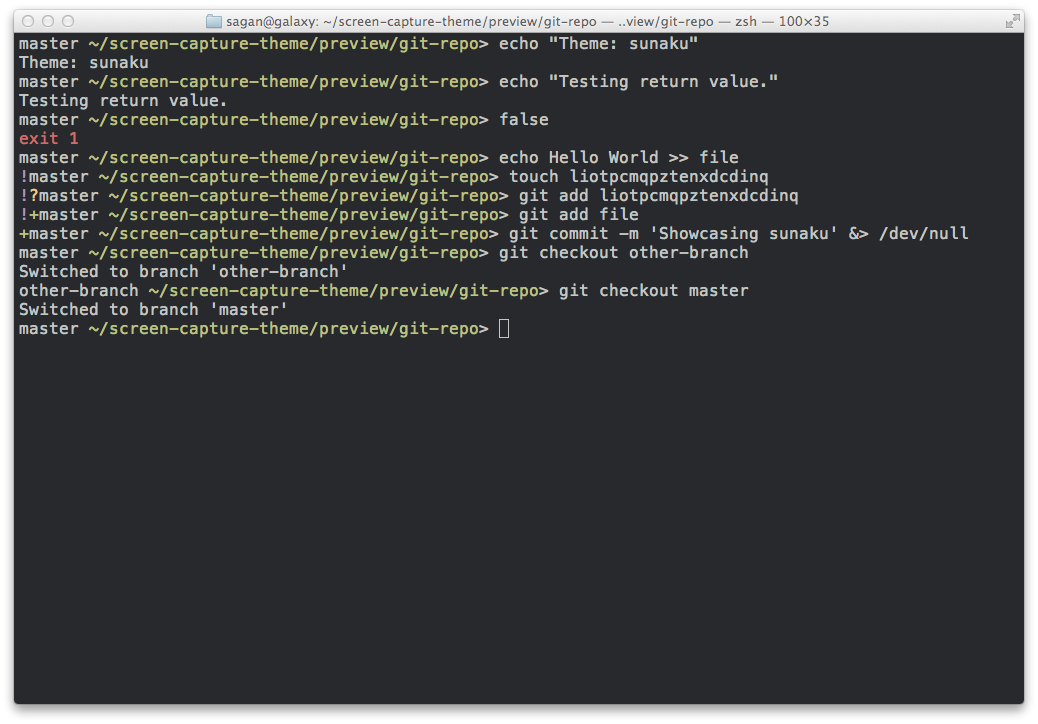
\includegraphics[scale=0.4]{sunaku.png}

\end{center}
\item Utilize um editor de texto com extensões para te ajudar a visualizar modificações no seu repositório enquanto você modifica o código, por exemplo Atom e vim

\end{itemize}

\subsection{DEU MERDA!!!} 

Tá tudo bem, você pode sobrescrever as alterações locais do seu repositório:
\begin{flushleft}
		\textit{\$ git checkout $--$ <nome do arquivo que você quer resetar>}
\end{flushleft}
Isso vai resetar as modificações do arquivo para como ele estava no último commit do branch atual. É por isso que é MUITO IMPORTANTE manter o costume de dar commits organizados e com código minimamente testado.
 
Se deu muita merda mesmo e você quer resetar o repositório local e recomeçar de onde você parou na origin, você pode fazer isso: 
\begin{flushleft}
\textit{\$ git fetch origin \newline
\$ git reset $--$hard origin/master}
\end{flushleft}

Isso vai buscar a última versão do repositório remoto origin e depois mandar o git resetar tudo do repositório local para o estado atual da origin. Por isso que é AINDA MAIS IMPORTANTE ser cuidadoso com os pushs para a origin.

\section{Github}
\subsection{Conta com email da Unicamp}
O Github é lindo, mas em contas FREE ele não permite que você faça repositórios fechados, o que é péssimo para seus trabalhos individuais. Por sorte, é possível utilizar o email da unicamp para ter acesso aos repositórios privados de graça!
\begin{itemize}
\item Crie uma conta no Github com qualquer email
\item Adicione seu gmail da dac (<primeira letra do seu nome><seu ra>@g.unicamp.br) à sua conta do Github em \textit{Personal Settings > Emails > Add email address } (se você usou ele no cadastro pule essa etapa) 
\item Entre nesse \href{https://education.github.com/pack/offers}{link}, ache a opção do Github e escolha a opção \textit{Get direct access on the GitHub website}. Depois siga os passos do link.
\end{itemize}

\subsection{Instruções gerais do Github}
\begin{itemize}
\item Mantenha um README um LICENÇA nos repositórios do github, você nunca sabe se alguém está interessado no seu código
\item Para criar um repositório remoto para um repositório local (ou seja, criar uma origin pro seu repositório local):
	\begin{enumerate}
	\item	 Siga as instruções do próprio Github para criar um novo projeto, por exemplo: \textit{repo-remoto}
	\item O Github vai fornecer alguns jeitos de adicionar coisas no repositório. Se você já possui um repositório local, basta copiar a url do repositório remoto que você acabou de criar (com o .git no final), vai ser algo como: \textit{https://github.com/seuusuario/repo-remoto.git}
	\item Depois, siga o passo 2 da seção \ref{comandos}
	\end{enumerate}
\end{itemize}

\section{Links úteis}
\begin{itemize}
\item Tutorial básico bem explicado: \url{http://rogerdudler.github.io/git-guide/index.pt_BR.html}
\item Introdução a repositórios do github: \url{https://guides.github.com/activities/hello-world/}
\item Readme lindo do Chams: \url{https://github.com/mrtheduts/readmegit}

\end{itemize}


\end{doublespacing}
\end{document}